\documentclass[letterpaper, 12pt]{article}
% \usepackage[showframe, margin=1in, top=0.25in, bottom=0.25in, includeheadfoot, headheight=0.5in]{geometry}
\usepackage[margin=1in, top=0.25in, bottom=0.25in, includeheadfoot, headheight=0.5in]{geometry}

\AddToHook{cmd/section/before}{\clearpage}

\usepackage[table]{xcolor}
\colorlet{listingback}{gray!20}
\definecolor{headingcolor}{RGB}{110,34,54}

\usepackage{fancyhdr}
\renewcommand{\sectionmark}[1]{\markboth{#1}{#1}}

% Used to detect whether a section is an appendix to print the right thing in the footer
\usepackage{etoolbox}
\newtoggle{inappendix}
\pretocmd{\appendix}{\clearpage\toggletrue{inappendix}}{}{}

% Save standard definitions for head and foot rules (lines separating header and footer from text)
\let\HeadRule\headrule
\let\FootRule\footrule
% Add color to the standard definitions
\renewcommand{\headrule}{\color{headingcolor}\HeadRule}
\renewcommand{\footrule}{\textcolor{headingcolor}{\FootRule}}

% IMPORTANT: This command should not be called directly. Use \preamble.
% Macro to insert the title page for each lab.
% The argument is the title of the lab.
\newcommand{\inserttitlepage}[1]
{
    \begin{titlepage}
    \centering
    
\includegraphics[scale=0.5]{images/nexus_lab_logo.png}

    \vspace*{\baselineskip}

    \textbf{\Large OpenStack Labs}

    \vspace*{\baselineskip}

    \textbf{\Large #1}
    \vspace*{\fill}
\end{titlepage}
}

% IMPORTANT: This command should not be called directly. Use \preamble.
% Macro to define header and footer for each lab.
% The argument is the title of the lab.
\newcommand{\headfoot}[1]
{
    \fancypagestyle{fancy}
    {
        \fancyhf{}
        \fancyhead[L]{\footnotesize #1}
        \fancyhead[R]{
\includegraphics[height=0.85\headheight]{images/nexus_lab_logo.png}}
        \fancyfoot[L]{%
            \footnotesize%
            \ifnum\value{section}>0%
            \iftoggle{inappendix}{Appendix \thesection: \rightmark}{Section \thesection: \rightmark}%
            \fi}
        \fancyfoot[R]{\footnotesize\thepage}
        \renewcommand{\headrulewidth}{1.5pt}
        \renewcommand{\footrulewidth}{1.5pt}
    }
}

% Macro to insert title page, define header and footer, and insert table of contents and about section for each lab.
% The argument is the title of the lab.
\newcommand{\preamble}[1]
{
    \pagenumbering{roman}
    \inserttitlepage{#1}
    \headfoot{#1}

    % Insert table of contents
    \pagestyle{fancy}
    \tableofcontents
    \clearpage

    \section*{About This Document}
    \label{sec:about_this_document}
    \begin{itemize}
        \item This document was developed by a team at the University of Tennessee at Chattanooga led by Dr. Mengjun Xie
        (\href{mailto:mengjun-xie@utc.edu}{\textbf{mengjun-xie@utc.edu}}).
        \item The development of this document was supported by a National Centers of Academic Excellence in Cybersecurity Grant (\#H98230-20-1-0351), housed at the National Security Agency.
        \item This document is licensed with a Creative Commons Attribution 4.0 International License.
    \end{itemize}
    \clearpage
}

% Macro to insert the Lab Settings page for each lab. Call after the Introduction and Objectives sections.
\newcommand{\labsettings}
{
    \section*{Lab Settings}
    \label{sec:lab_settings}
    \addcontentsline{toc}{section}{\nameref{sec:lab_settings}}
    The information in the table below will be needed in order to complete the lab.
    The task sections below provide details on the use of this information.
    \begin{table*}[htbp]
        \centering
        \begin{tabular}{|c|c|c|c|}
            \hline
            \rowcolor{gray!20} \textbf{Virtual Machine} & \textbf{IP Address} & \textbf{Account} & \textbf{Password} \\
            \hline
            \multirow{2}{*}{\texttt{workstation}} & \multirow[t]{2}{*}{\texttt{ens3: 192.168.1.21}}  & \multirow{2}{*}{\texttt{ubuntu}} & \multirow{2}{*}{\texttt{ubuntu}} \\
                                                  & \multirow[t]{2}{*}{\texttt{ens4: 172.25.250.21}} &                                  &                                  \\
            \hline
            \multirow{2}{*}{\texttt{devstack}}    & \multirow[t]{2}{*}{\texttt{ens3: 192.168.20}}    & \multirow{2}{*}{\texttt{ubuntu}} & \multirow{2}{*}{\texttt{ubuntu}} \\
                                                  & \multirow[t]{2}{*}{\texttt{ens4: 172.25.250.20}} &                                  &                                  \\
            \hline
        \end{tabular}
    \end{table*}
    \clearpage

    % IMPORTANT(lucas): If another frontmatter section ever gets placed after this, this command needs to be moved
    % to the end of that section.
    % I have placed this here and not in each lab purely for convenience and to ensure I don't forget any.
    \pagenumbering{arabic}
}

% Sans-serif font
\renewcommand{\familydefault}{\sfdefault}
\newcommand{\texttildemid}{{\raisebox{0.5ex}{\texttildelow}}}

\usepackage{enumitem}
\renewcommand{\labelenumi}{\textbf{\thesection.\arabic{enumi}.}}

% Try to forbid widows and orphans
\widowpenalty10000
\clubpenalty10000

\usepackage{graphicx}
\usepackage{hyperref}
\hypersetup{colorlinks=true,linkcolor=black,urlcolor={[named] headingcolor}}

\usepackage{sectsty}
\sectionfont{\color{headingcolor}}

% Table of Contents
\usepackage{bookmark}
\usepackage[titles]{tocloft}
\usepackage[title]{appendix}
\renewcommand{\cfttoctitlefont}{\Large\bfseries\color{headingcolor}}
\renewcommand{\cftsecfont}{\normalfont\normalsize}
\renewcommand{\cftsecpagefont}{\normalfont\normalsize}
\renewcommand{\cftdotsep}{0} % Make dots small and close together
\renewcommand{\cftsecleader}{\cftdotfill{\cftdotsep}} % Add dots after section titles
% Make dots go all the way to the page number
\renewcommand{\cftsecfillnum}[1]{{\cftsecleader}\nobreak{\cftsecpagefont #1}\cftsecafterpnum\par}

\usepackage{multirow}
\setlength{\tabcolsep}{16pt}
\renewcommand{\arraystretch}{1.1}

% For nice-looking boxes
\usepackage[most]{tcolorbox}
\usepackage{listings}
\usepackage{lstautogobble}
\lstset{
  frame=none,
  language=Bash,
  showstringspaces=false,
  basicstyle={\linespread{1.1}\footnotesize\ttfamily\selectfont},
  numbers=none,
  breaklines=true,
  breakatwhitespace=true,
  tabsize=3,
  columns=fullflexible,
  keepspaces=true,
  escapeinside={(*@}{@*)},
  literate={~}{{\texttildemid}}{1}
           {\#}{\#}{1},
  autogobble=true
}

\tcolorboxenvironment{lstlisting}
{
    spartan,
    colframe=gray!50,
    boxsep=0mm,
    left=1mm,
    right=1mm,
    top=-1mm,
    bottom=-1mm,
    colback=gray!20
}

% Hacky solution for now, would like to have just one environment and make several tcolorboxes by passing different
% colors as parameters, but that is giving errors
\makeatletter
\tcbset{
  note/.style={%
        enhanced,
        breakable,
        colback=blue!10!white,
        colframe=blue!80!white,
        attach boxed title to top left={yshift*=-\tcboxedtitleheight},
        title={#1},
        boxed title size=title,
        boxed title style={%
            sharp corners,
            rounded corners=northwest,
            colback=tcbcolframe,
            boxrule=0pt,
        },
        underlay boxed title={%
            \path[fill=tcbcolframe] (title.south west)--(title.south east)
                to[out=0, in=180] ([xshift=5mm]title.east)--
                (title.center-|frame.east)
                [rounded corners=\kvtcb@arc] |-
                (frame.north) -| cycle;
        },
    }
}
\makeatother

\makeatletter
\tcbset{
    stop/.style={%
        enhanced,
        breakable,
        colback=white,
        colback=red!10!white,
        colframe=red!80!white,
        attach boxed title to top left={yshift*=-\tcboxedtitleheight},
        title={#1},
        boxed title size=title,
        boxed title style={%
            sharp corners,
            rounded corners=northwest,
            colback=tcbcolframe,
            boxrule=0pt,
        },
        underlay boxed title={%
            \path[fill=tcbcolframe] (title.south west)--(title.south east)
                to[out=0, in=180] ([xshift=5mm]title.east)--
                (title.center-|frame.east)
                [rounded corners=\kvtcb@arc] |-
                (frame.north) -| cycle;
        },
    }
}
\makeatother

\makeatletter
\tcbset{
    tip/.style={%
        enhanced,
        breakable,
        colback=white,
        colback=green!10,
        colframe=green!70!black,
        attach boxed title to top left={yshift*=-\tcboxedtitleheight},
        fonttitle=\bfseries,
        title={#1},
        boxed title size=title,
        boxed title style={%
            sharp corners,
            rounded corners=northwest,
            colback=tcbcolframe,
            boxrule=0pt,
        },
        underlay boxed title={%
            \path[fill=tcbcolframe] (title.south west)--(title.south east)
                to[out=0, in=180] ([xshift=5mm]title.east)--
                (title.center-|frame.east)
                [rounded corners=\kvtcb@arc] |-
                (frame.north) -| cycle;
        },
    }
}
\makeatother

% The commands below define environments for colored boxes. They are used like
% \begin{notebox}
% ...
% \end{notebox}
\newtcolorbox{notebox}{note={Note}}
\newtcolorbox{stopbox}{stop={Stop}}
\newtcolorbox{tipbox}{tip={Tip}}

\begin{document}
\preamble{Lab 01: Launching an Instance}

\section*{Introduction}
\label{sec:introduction}
\addcontentsline{toc}{section}{\nameref{sec:introduction}}
In this lab, you will launch an instance using the \textit{Horizon Dashboard}, launch an instance using the
\textit{OpenStack Unified CLI}, and use the \textit{OpenStack Unified CLI}.

\section*{Objectives}
\label{sec:objectives}
\addcontentsline{toc}{section}{\nameref{sec:objectives}}
\begin{itemize}[itemsep=0pt]
    \item Use the \textit{Horizon Dashboard}.
    \item Launch an instance using the \textit{Horizon Dashboard}.
    \item Use the \textit{OpenStack Unified CLI}.
    \item Launch an instance using the \textit{OpenStack Unified CLI}.
\end{itemize}
\clearpage

\labsettings

%%%%%%%%%%%
% Section 1
%%%%%%%%%%%
\section{Launching an Instance Using the Horizon Dashboard}
In this task, you will launch an instance using the \textit{Horizon Dashboard}.

\begin{enumerate}
    \item Log into the \textbf{workstation} machine as the \textbf{ubuntu} user with password \textbf{ubuntu}.

    \begin{center}
        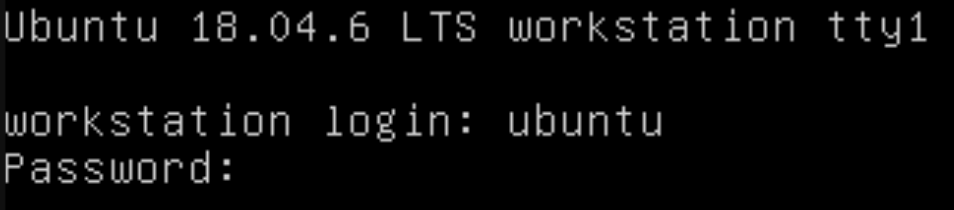
\includegraphics[width=\linewidth]{images/part1/step1.png}
    \end{center}

    \item Launch the graphical user interface.
    \begin{lstlisting}
        ubuntu@workstation:~$ startx
    \end{lstlisting}

    \begin{center}
        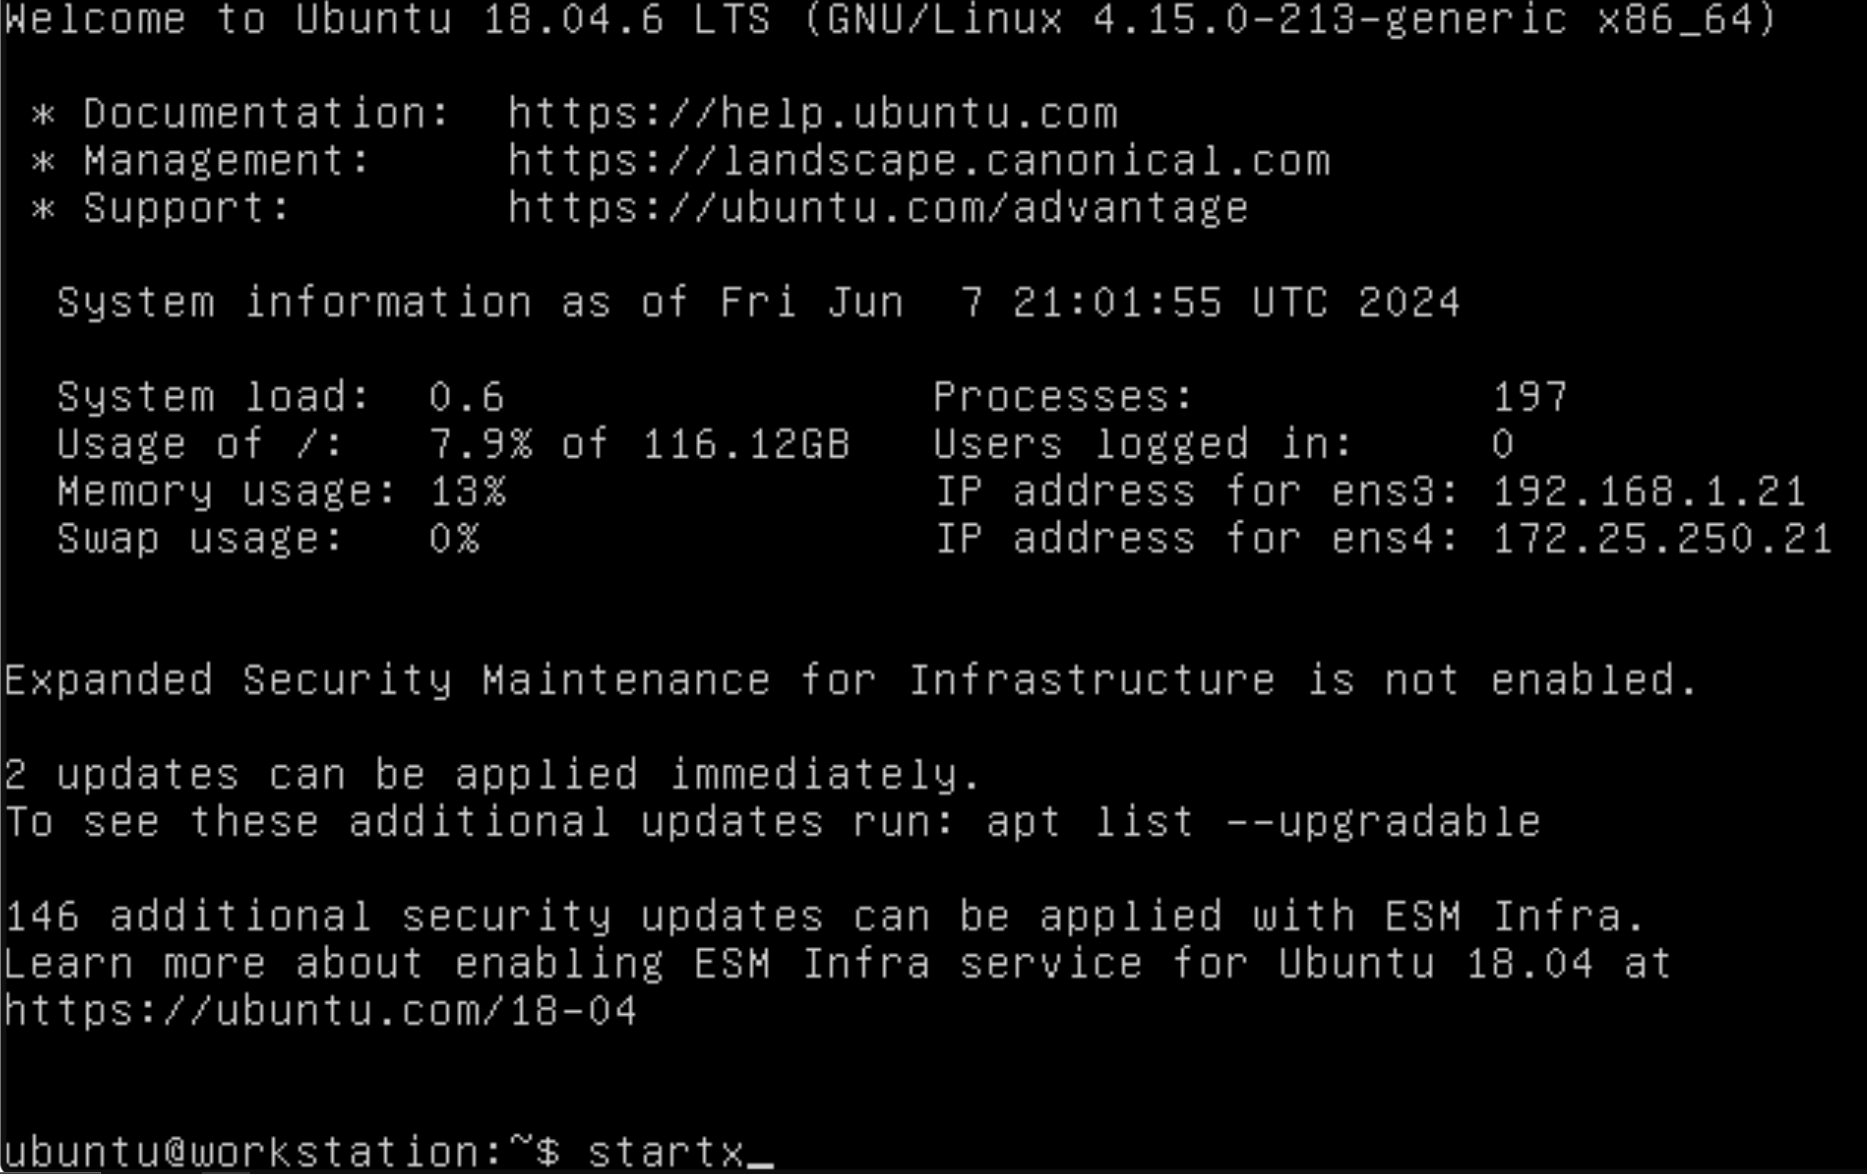
\includegraphics[width=\linewidth]{images/part1/step2.png}
    \end{center}

    \item Open the web browser.

    \begin{center}
    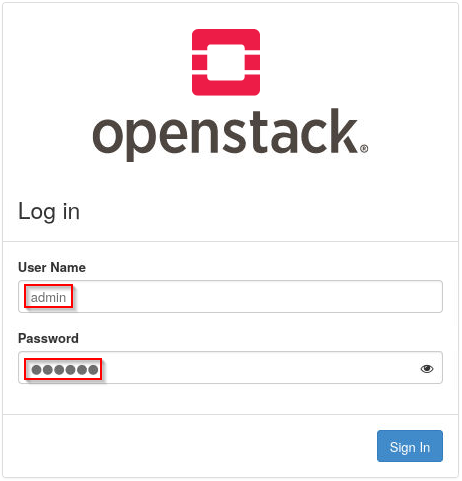
\includegraphics[scale=0.75]{images/part1/step3.png}
    \end{center}

    \item Enter the IP address of the \textbf{devstack} machine (\textbf{192.168.1.20}) into the address bar, and log
    into the OpenStack Horizon Dashboard. The username is \textbf{admin} and the password is \textbf{secret}.
    
    \begin{center}
        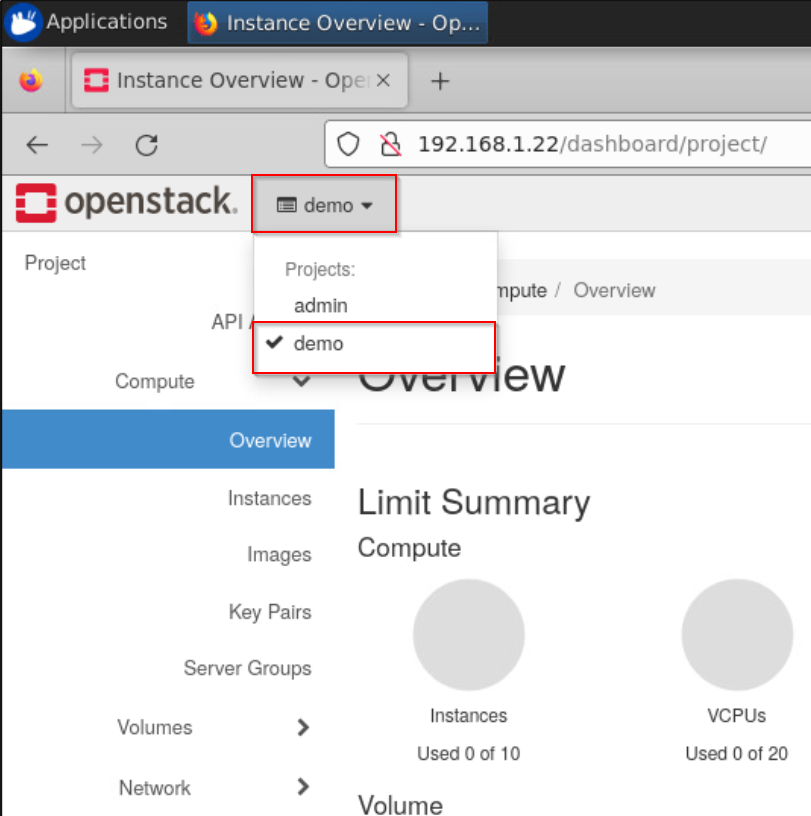
\includegraphics[scale=0.65]{images/part1/step4.png}
    \end{center}

    \item Click on the dropdown menu in the top left corner of the webpage, then select \textbf{demo} as the project.
    Navigate to \textbf{Project $>$ Compute $>$ Instances}, then click \textbf{Launch Instance} in the top right corner.

    \begin{center}
        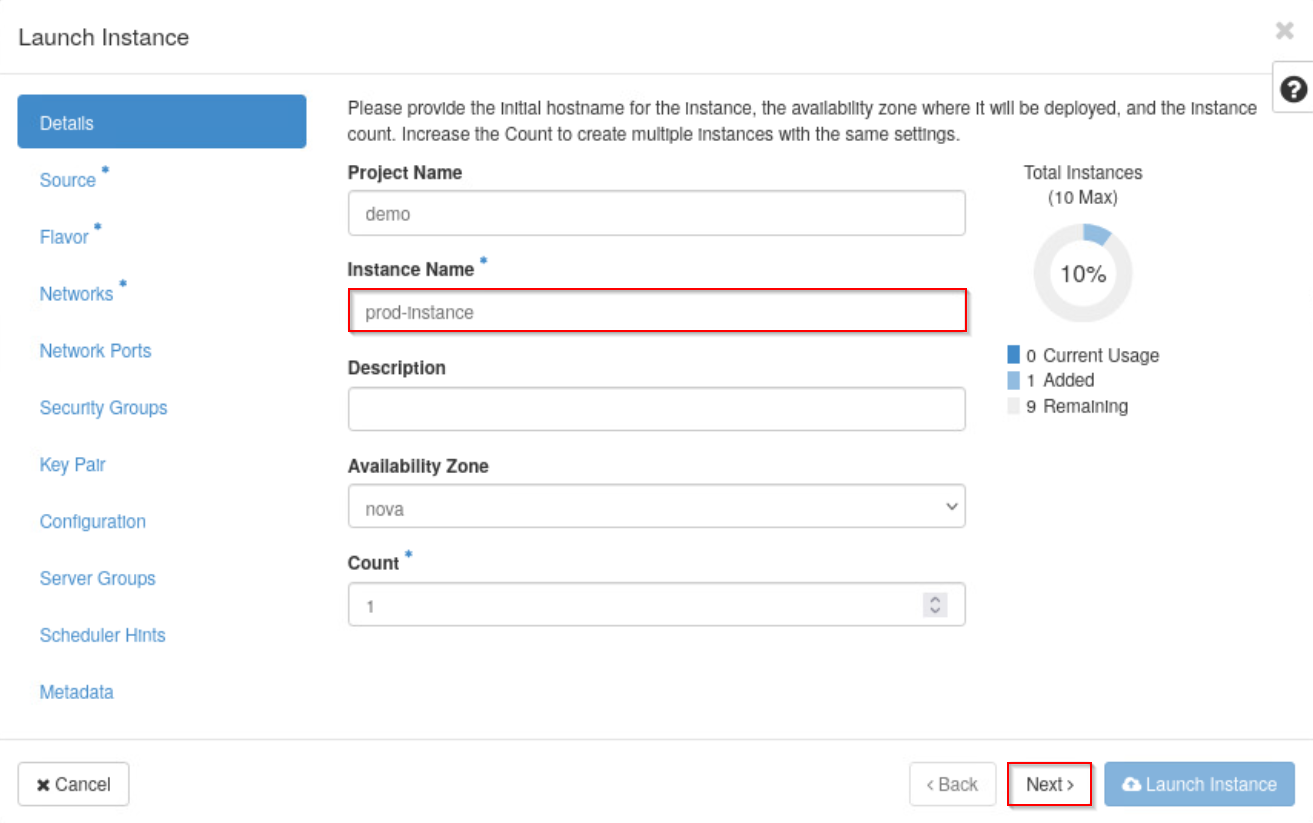
\includegraphics[width=\linewidth]{images/part1/step5.png}
    \end{center}

    \item In the \textit{Instance Name} field, type \textbf{prod-instance}, and leave the other fields with their
    default values. Click \textbf{Next}.

    \begin{center}
        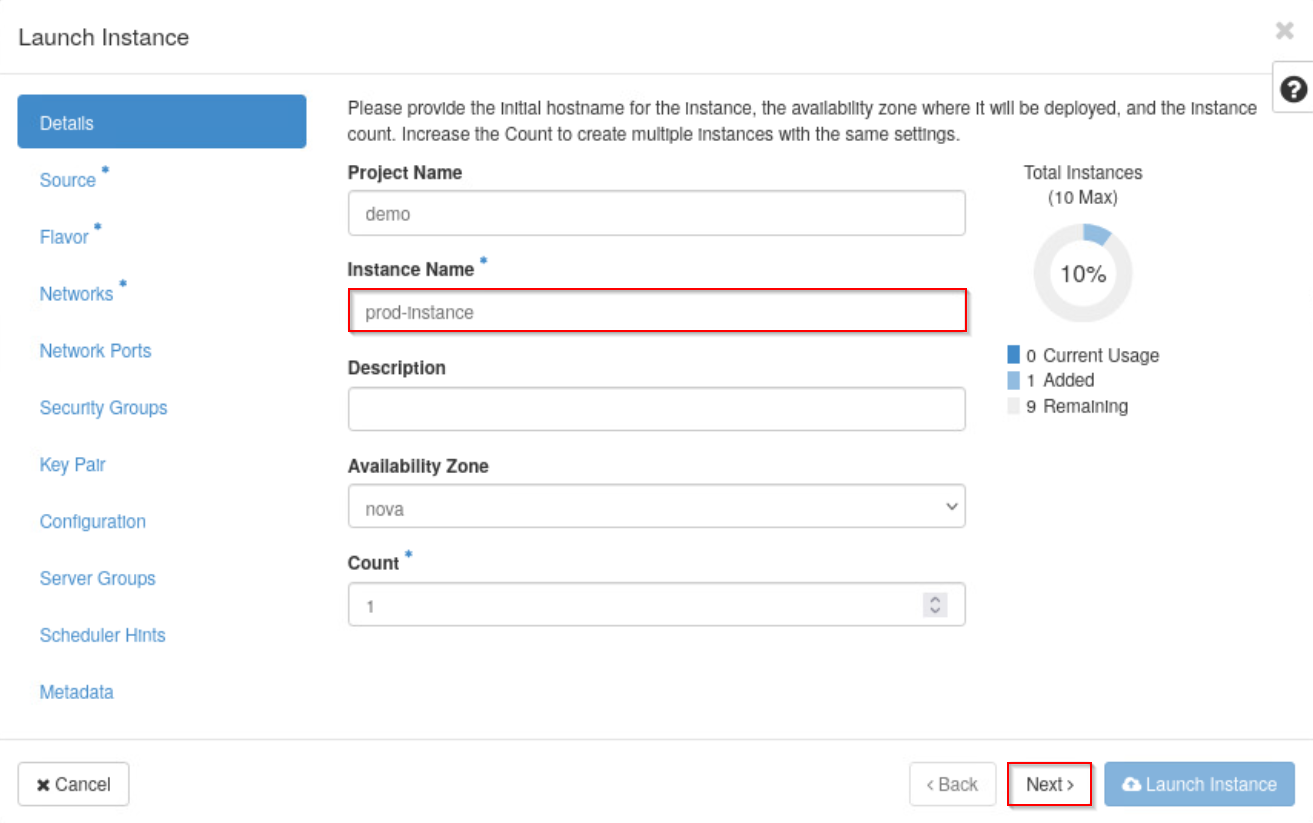
\includegraphics[width=\linewidth]{images/part1/step6.png}
    \end{center}

    \item In the \textit{Select Boot Source} drop dow, select \textbf{Image}, set \textit{Create New Volume} to
    \textbf{No} and scroll down (if needed) to click the $\uparrow$ icon beside of \textbf{ubuntu} to use
    \textbf{ubuntu} as the image. Click \textbf{Next}.

    \begin{center}
        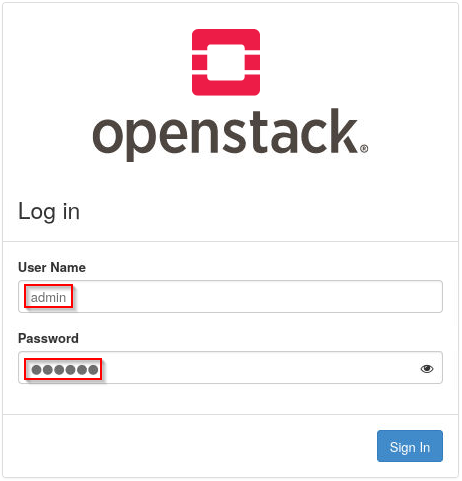
\includegraphics[width=\linewidth]{images/part1/step7.png}
    \end{center}

    \begin{stopbox}
        Before proceeding to the next step, confirm that \textbf{ubuntu} appears underneath the \textit{Allocated}
        section.
    \end{stopbox}
    
    \item Scroll down (if needed) and click the $\uparrow$ icon beside the \textbf{m1.small} flavor. Click
    \textbf{Next}.
    
    \begin{center}
        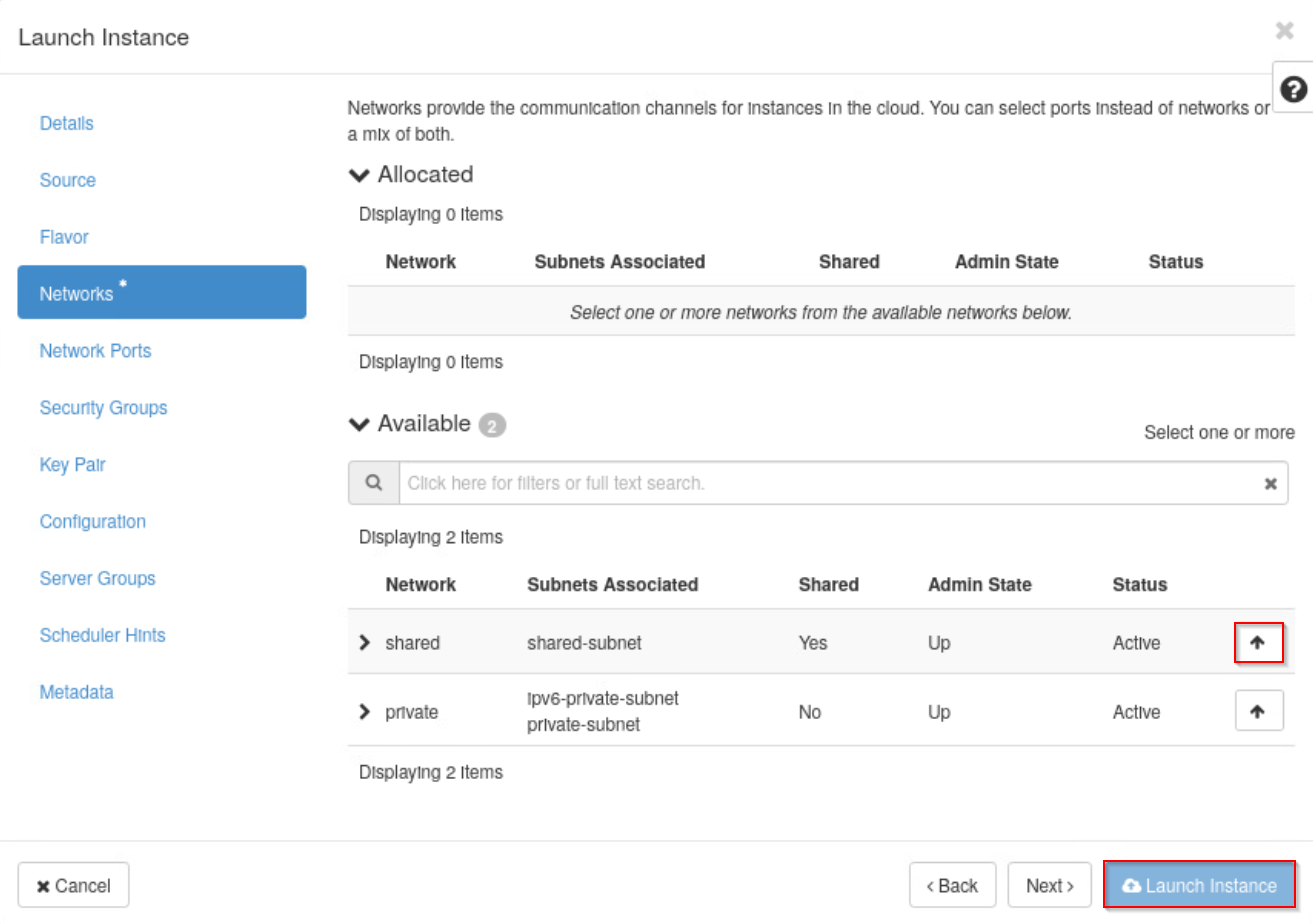
\includegraphics[width=\linewidth]{images/part1/step8.png}
    \end{center}

    \begin{stopbox}
        Before proceeding to the next step, confirm that \textbf{m1.small} appears underneath the \textit{Allocated}
        section.
    \end{stopbox}

    \item Click the $\uparrow$ icon beside the \textbf{shared} network. If all required fields have been set, the
    \textbf{Launch Instance} button in the bottom right corner should now be clickable. Click \textbf{Launch Instance}.

    \begin{center}
        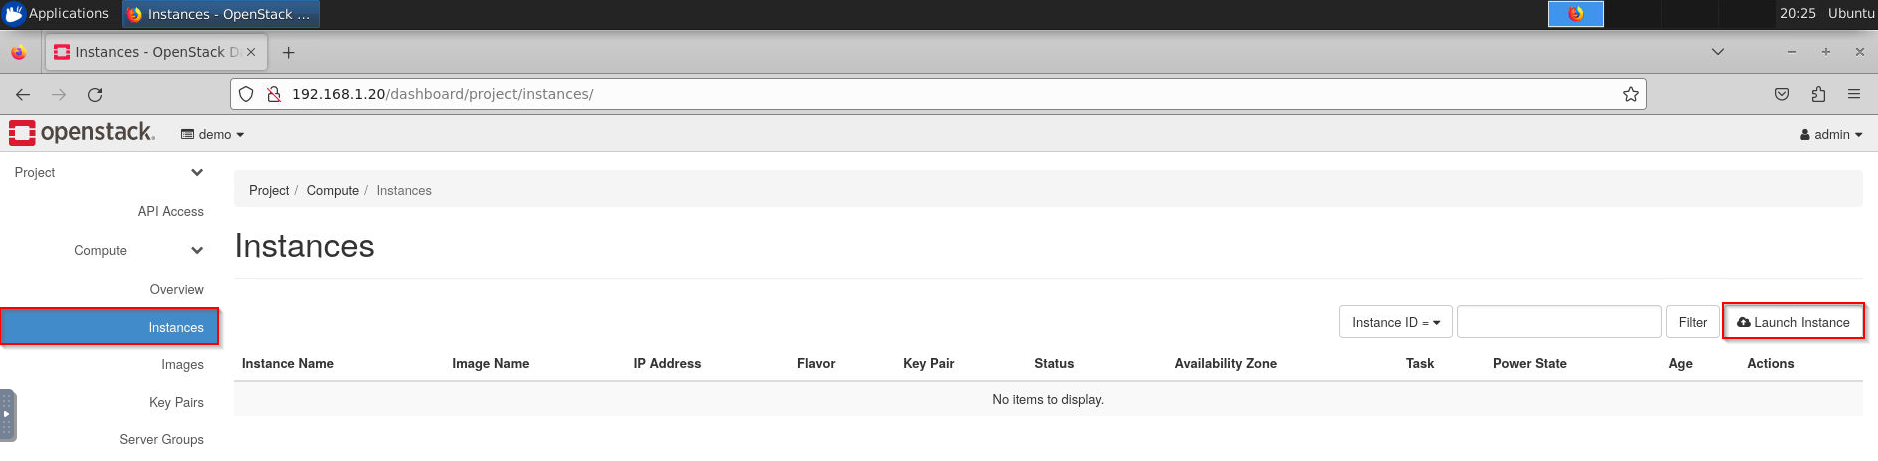
\includegraphics[width=\linewidth]{images/part1/step9.png}
    \end{center}

    \begin{stopbox}
        Before proceeding to the next step, confirm that \textbf{shared} appears underneath the \textit{Allocated}
        section.
    \end{stopbox}

    \item To open the console of \textbf{prod-instance} in a new tab, right-click on the name \textbf{prod-instance} and
    select \textbf{Open Link in New Tab}, or middle-click (press in the mouse wheel) the name \textbf{prod-instance}.

    \begin{center}
        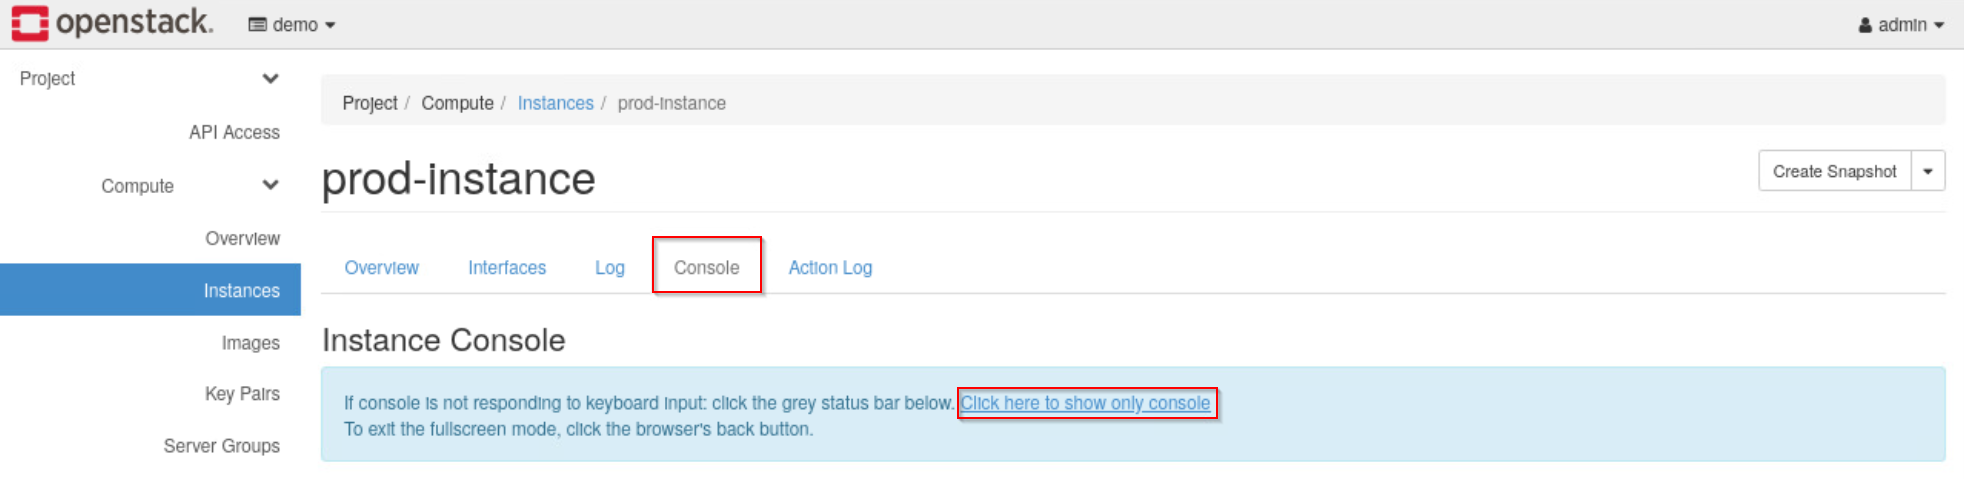
\includegraphics[width=\linewidth]{images/part1/step10.png}
    \end{center}

    \begin{stopbox}
        Wait for the \textit{Power State} of \textbf{prod-instance} to display the status of \textit{Running} before
        continuing to the next step.
    \end{stopbox}

    \item In the new tab, click the \textit{Console} tab. Optionally, to make the console take up the whole tab, click
    the \textbf{Click here to show only console} link.
    
    \begin{center}
        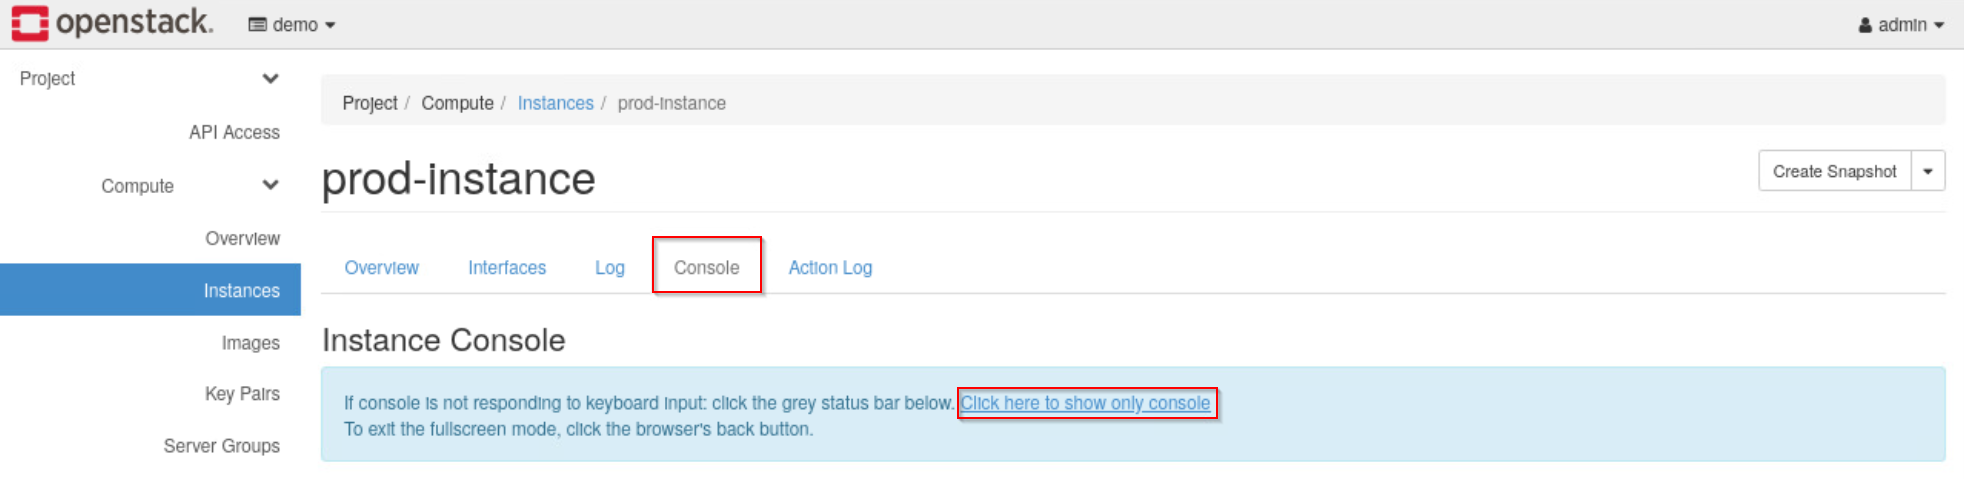
\includegraphics[width=\linewidth]{images/part1/step11.png}
    \end{center}

    \item Log into the console as \textbf{root} with the password \textbf{secret}.
    
    \begin{notebox}
        It may take several minutes for the instance to fully boot up and present a login prompt.
    \end{notebox}

    \item In the console, ping \textbf{192.168.233.2} (DHCP server) to verify connectivity.
    \begin{lstlisting}
        $ ping -c3 192.168.233.2
    \end{lstlisting}

    \begin{center}
        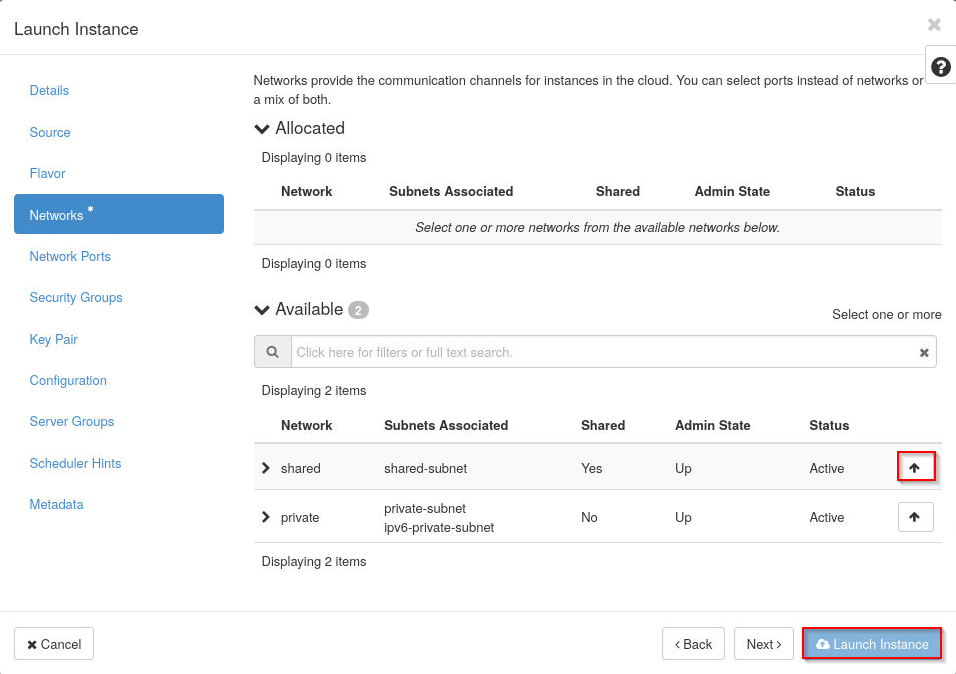
\includegraphics[width=\linewidth]{images/part1/step13.png}
    \end{center}

    \begin{notebox}
        You should receive three successful ping replies.
    \end{notebox}

    \item Close the console tab for \textbf{prod-instance}.

    \item Focus back on the tab showing instances and delete \textbf{prod-instance}. Select the checkbox for
    \textbf{prod-instance} and click the \textbf{Delete Instances} button.

    \begin{center}
        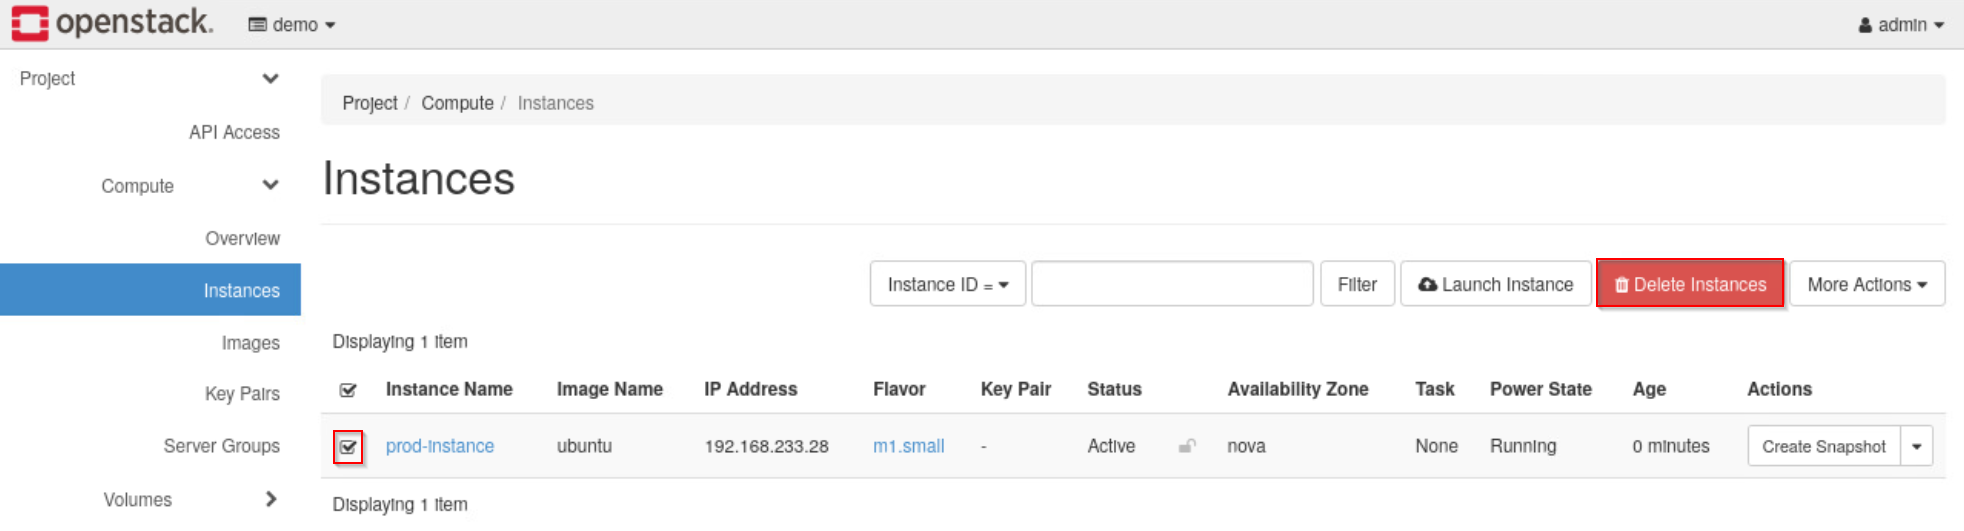
\includegraphics[width=\linewidth]{images/part1/step15.png}
    \end{center}

    \item Confirm the deletion by clicking the \textbf{Delete Instances} button.

    \begin{center}
        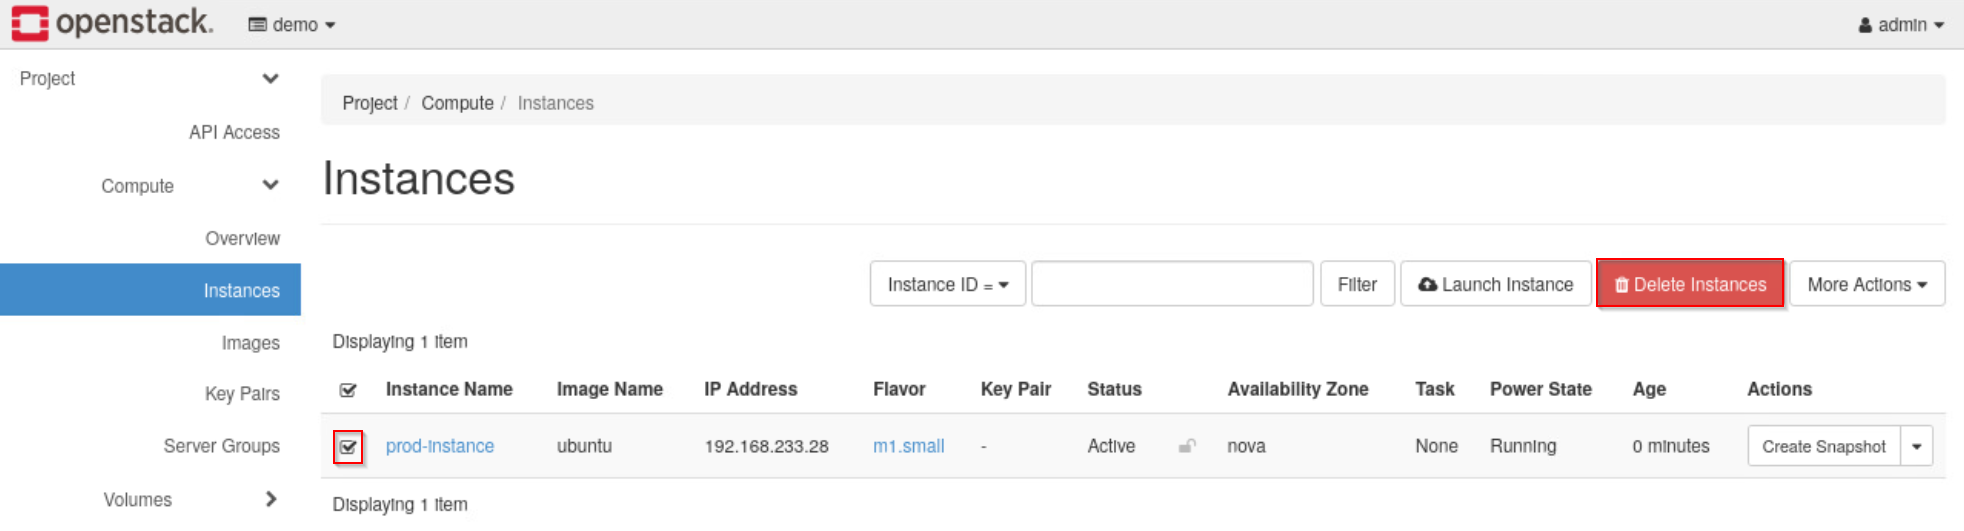
\includegraphics[width=\linewidth]{images/part1/step16.png}
    \end{center}

    \item Close the web browser.
\end{enumerate}

%%%%%%%%%%%
% Section 2
%%%%%%%%%%%
\section{Running the OpenStack Unified CLI}
In this task, you will use the \textit{OpenStack Unified command-line interface (CLI)} to list and check the details of
existing projects, users, flavors, images, and instances, and to launch an instance.

\begin{enumerate}
    \item Open a terminal, either by right-clicking the desktop and selecting \textbf{Open Terminal Here}, by clicking
    the terminal icon in the icon bar at the bottom of the screen, or by selecting \textbf{Applications} at the top
    left of the screen, then selecting \textbf{Terminal Emulator}.

    \begin{center}
        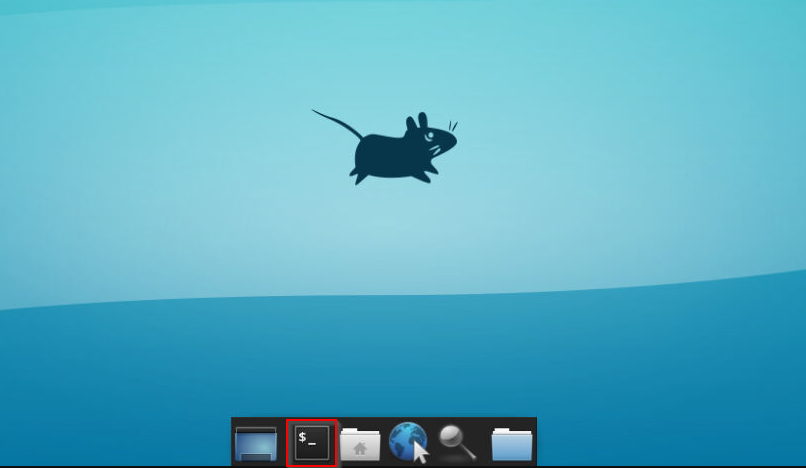
\includegraphics[width=\linewidth]{images/part2/step1.png}
    \end{center}

    \item The \textbf{keystonerc-admin} file in the home directory defines several \textbf{OS\_*} environment variables
    that allow you to use the OpenStack platform on the \textbf{devstack} server through the OpenStack Unified CLI. Th
     username will be \textbf{admin}, the password will be be \textbf{secret}, the project will be \textbf{demo}, and
     the IP address for \textbf{OS\_AUTH\_URL} is the IP address of the \textbf{devstack} server, \textbf{192.168.1.20}.
     You can run \textbf{cat} on the file to view its contents.
    \begin{lstlisting}
        ubuntu@workstation:~$ cat ~/keystonerc-admin
    \end{lstlisting}

    \begin{center}
        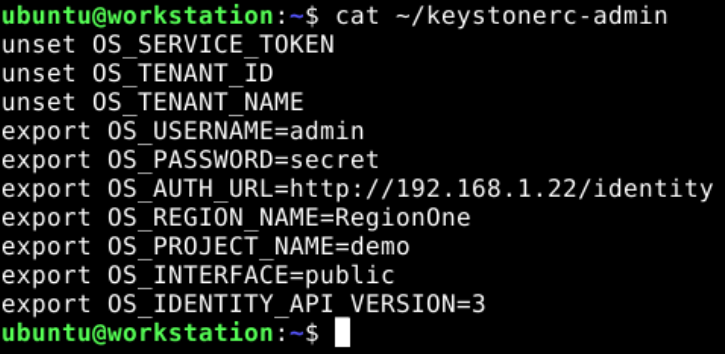
\includegraphics[width=\linewidth]{images/part2/step2.png}
    \end{center}

    \item Use the \textbf{source} command with the \textbf{keystonerc-admin} argument to enable all the
    \textbf{OS\_*} environment variables included in the \textbf{keystonerc-admin} file.
    \begin{lstlisting}
        ubuntu@workstation:~$ source ~/keystonerc-admin
    \end{lstlisting}

    \begin{center}
        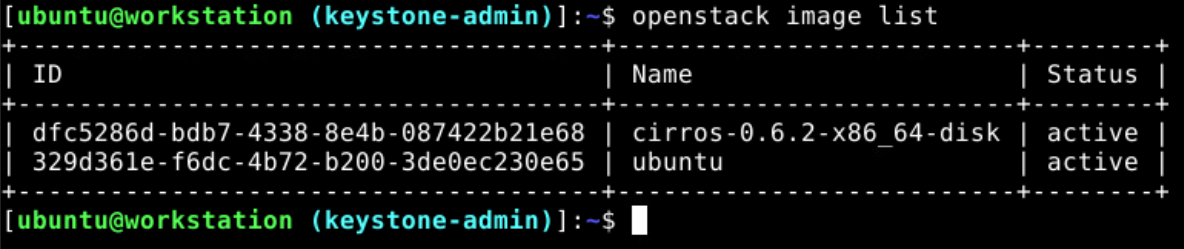
\includegraphics[width=\linewidth]{images/part2/step3.png}
    \end{center}
        
    \begin{notebox}
        The \textbf{export PS1=...} line at the end of the keystone credentials file modifies the shell prompt to show
        the OpenStack user whose credentials are keyed in. So, after running this command, you will notice that your
        shell prompt has changed to show you are keyed in as the \textbf{admin} user.
    \end{notebox}

    \begin{notebox}
        The same prompt without color can be achieved with the line
        \textbf{export PS1='[\textbackslash u@\textbackslash h (keystone-admin)]:\textbackslash w\$ '}. Here,
        \textbf{\textbackslash u} stands for the current username, \textbf{\textbackslash h} is the hostname, and
        \textbf{\textbackslash w} is the current working directory. The other escape sequences specify the colors of the
        prompt. For example, \textbf{\textbackslash[\textbackslash 033[01;32m\textbackslash]} sets the color to a light
        green, and \textbf{\textbackslash[\textbackslash 033[00m\textbackslash]} resets the color to the default
        (white in this case).
    \end{notebox}

    \item Verify that the \textbf{OS\_*} environment variables have been exported to the shell environment.
    \begin{lstlisting}
        [ubuntu@workstation (keystone-admin)]:~$ env | grep OS_
    \end{lstlisting}

    \begin{center}
        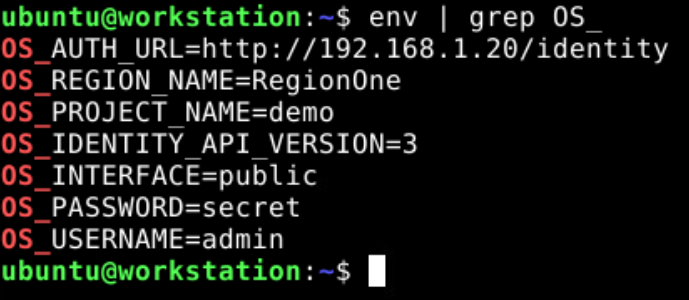
\includegraphics[width=\linewidth]{images/part2/step4.png}
    \end{center}

    \item Next, we will gather additional information about the users and projects. First, list the available projects.
    \begin{lstlisting}
        [ubuntu@workstation (keystone-admin)]:~$ openstack project list
    \end{lstlisting}

    \begin{center}
        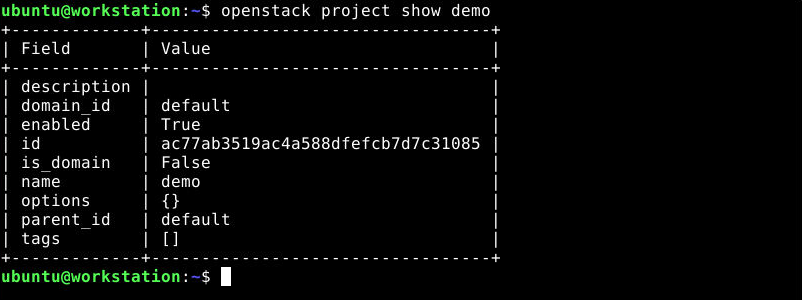
\includegraphics[width=\linewidth]{images/part2/step5.png}
    \end{center}

    \item Enter the command below to show more details about the \textbf{demo} project.
    \begin{lstlisting}
        [ubuntu@workstation (keystone-admin)]:~$ openstack project show demo
    \end{lstlisting}

    \begin{center}
        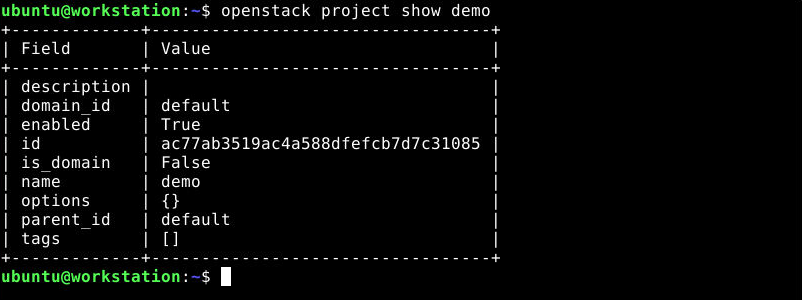
\includegraphics[width=\linewidth]{images/part2/step6.png}
    \end{center}

    \begin{notebox}
        Any ID values shown in these examples may differ from what you see since they are unique.
    \end{notebox}

    \begin{tipbox}
        Use the \textbf{openstack help project show} command to determine how to display the details of a particular
        project.
    \end{tipbox}

    \item List the available users.
    \begin{lstlisting}
        [ubuntu@workstation (keystone-admin)]:~$ openstack project user list
    \end{lstlisting}

    \begin{center}
        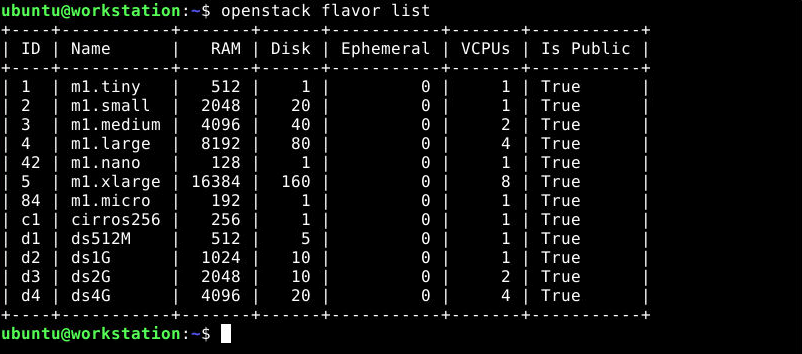
\includegraphics[width=\linewidth]{images/part2/step7.png}
    \end{center}

    \item Enter the command below to check the details of \textbf{admin}.
    \begin{lstlisting}
        [ubuntu@workstation (keystone-admin)]:~$ openstack user show admin
    \end{lstlisting}

    \begin{center}
        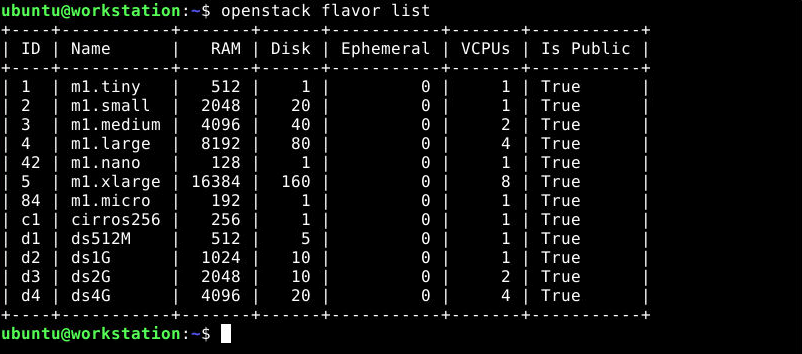
\includegraphics[width=\linewidth]{images/part2/step8.png}
    \end{center}

    \begin{tipbox}
        Use the \textbf{openstack help user show} command to determine how to display details of a specific user
        account.
    \end{tipbox}

    \item Enter the command below to list all available flavors.
    \begin{lstlisting}
        [ubuntu@workstation (keystone-admin)]:~$ openstack flavor list
    \end{lstlisting}

    \begin{center}
        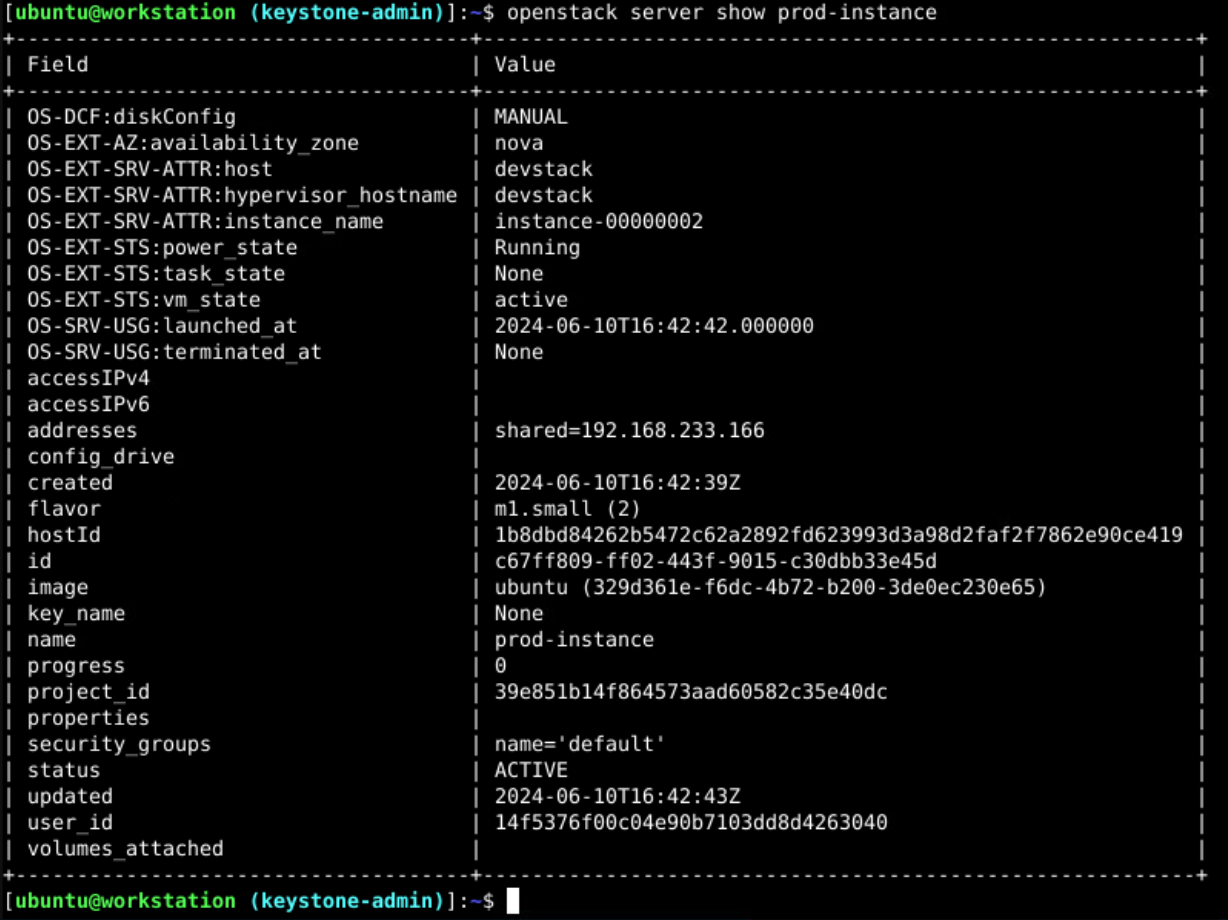
\includegraphics[width=\linewidth]{images/part2/step9.png}
    \end{center}

    \begin{tipbox}
        Use the \textbf{openstack help flavor list} command to determine how to display all available flavors.
    \end{tipbox}

    \item Enter the command below to display the details specifically for the \textbf{m1.small} flavor.
    \begin{lstlisting}
        [ubuntu@workstation (keystone-admin)]:~$ openstack flavor show m1.small
    \end{lstlisting}

    \begin{center}
        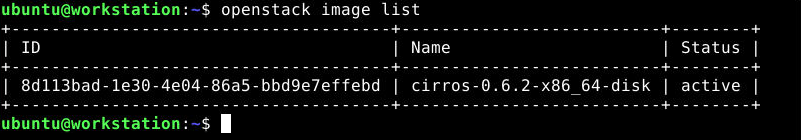
\includegraphics[width=\linewidth]{images/part2/step10.png}
    \end{center}

    \item Enter the command below to list all available images.
    \begin{lstlisting}
        [ubuntu@workstation (keystone-admin)]:~$ openstack image list
    \end{lstlisting}

    \begin{center}
        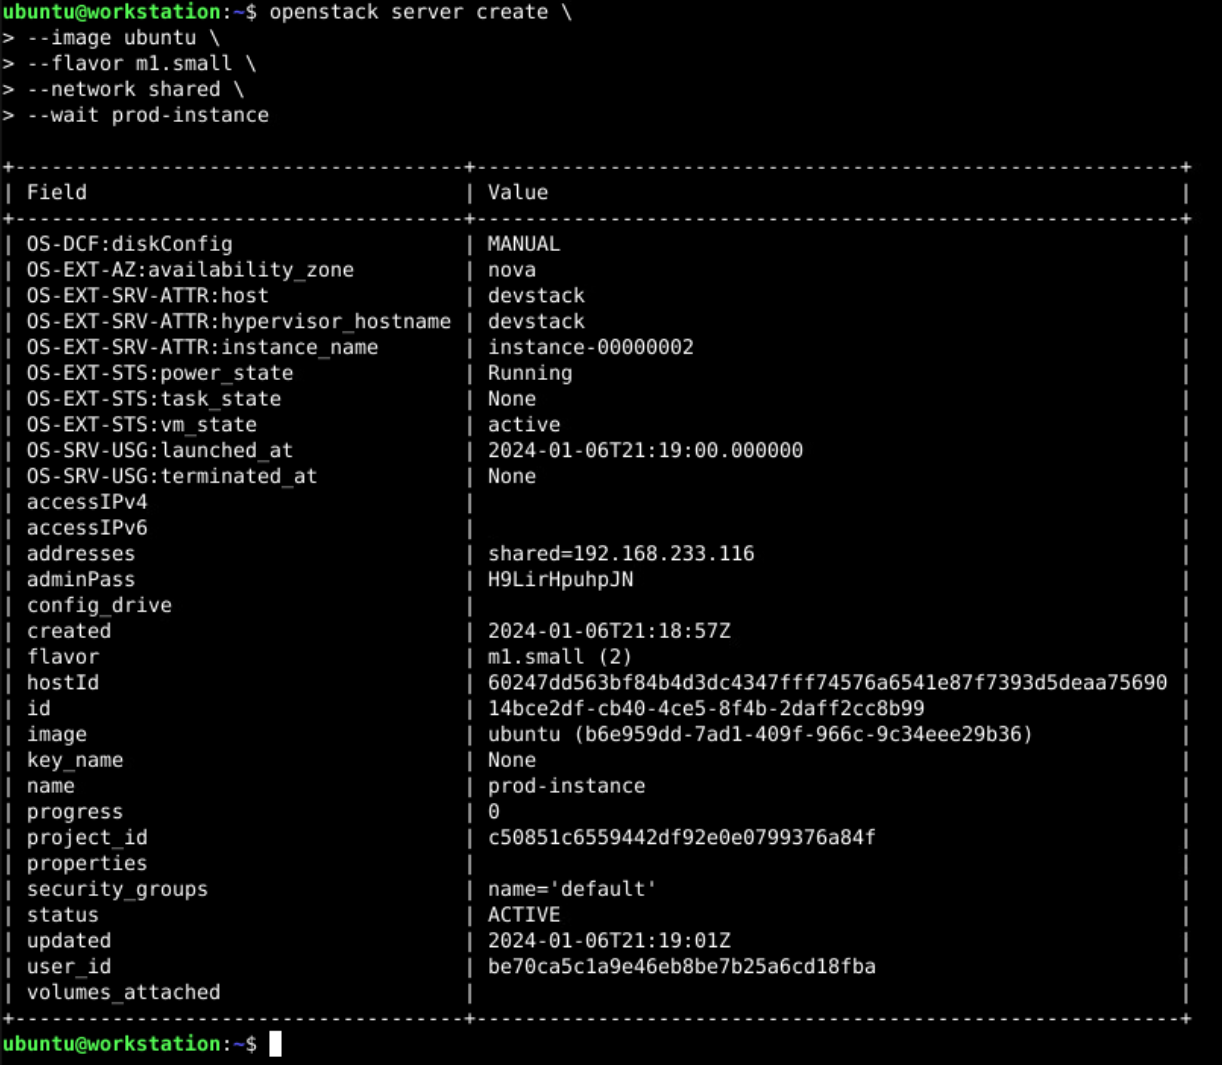
\includegraphics[width=\linewidth]{images/part2/step11.png}
    \end{center}

    \begin{tipbox}
        Use the \textbf{openstack help image} command to determine how to list all images.
    \end{tipbox}

    \item Enter the command below to list all available networks.
    \begin{lstlisting}
        [ubuntu@workstation (keystone-admin)]:~$ openstack network list
    \end{lstlisting}

    \begin{center}
        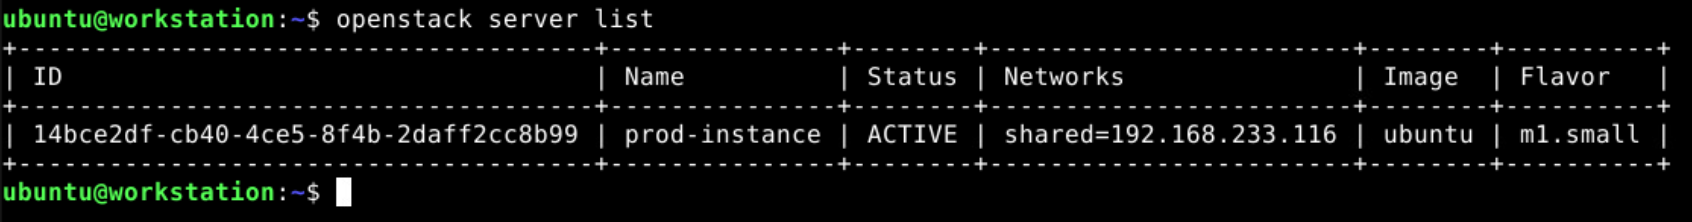
\includegraphics[width=\linewidth]{images/part2/step12.png}
    \end{center}

    \begin{tipbox}
        Use the \textbf{openstack help network} command to determine how to list all networks.
    \end{tipbox}

    \item Enter the command below to create a new instance with the name \textbf{prod-instance}, using
    \textbf{ubuntu} as the image, \textbf{m1.small} as the flavor, and \textbf{shared} as the network.
    \begin{lstlisting}
        [ubuntu@workstation (keystone-admin)]:~$ openstack server create \
        > --image ubuntu \
        > --flavor m1.small \
        > --network shared \
        > prod-instance
    \end{lstlisting}

    \begin{center}
        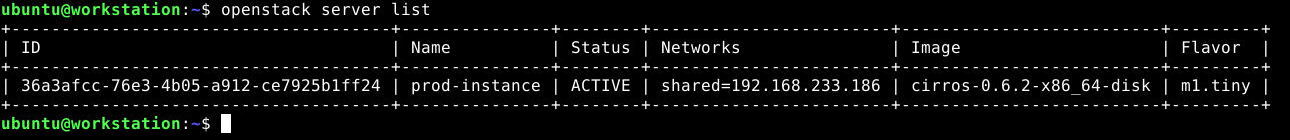
\includegraphics[width=\linewidth]{images/part2/step13.png}
    \end{center}

    \begin{tipbox}
        When typing the command, make sure there is a space between the last word of the line and the
        \textbf{\textbackslash}, and press \textbf{Enter} to get the \textbf{$>$} and continue typing the rest of the
        command.
    \end{tipbox}

    \item Use the \textbf{openstack server list} command to list all the available instances.
    \begin{lstlisting}
        [ubuntu@workstation (keystone-admin)]:~$ openstack server list
    \end{lstlisting}

    \begin{center}
        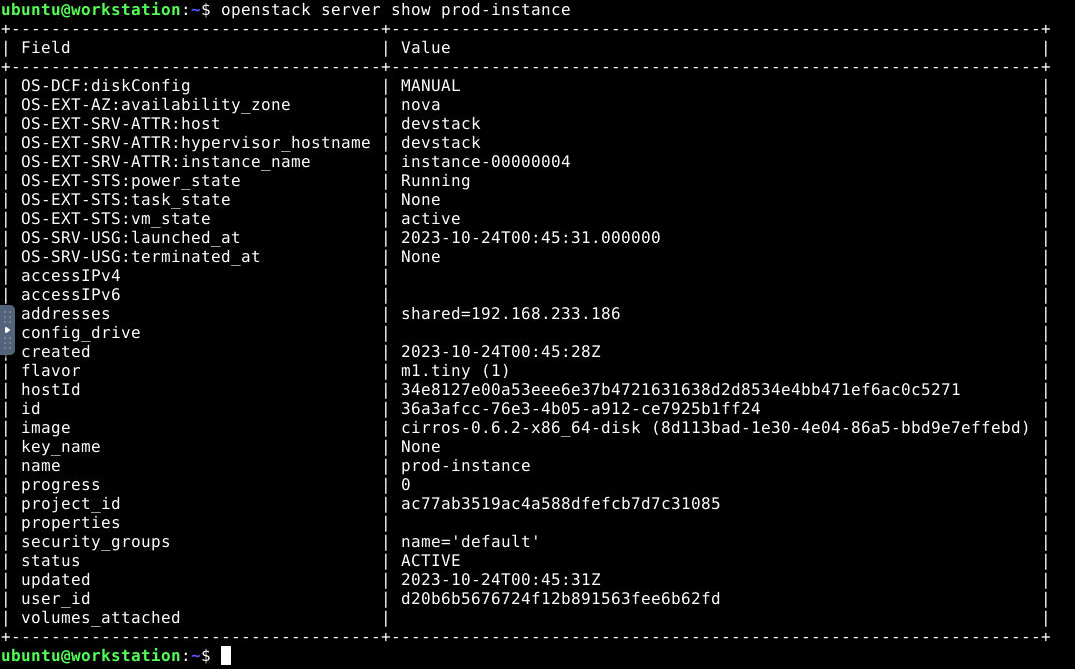
\includegraphics[width=\linewidth]{images/part2/step14.png}
    \end{center}

    \begin{notebox}
        The UUID in the \textit{ID} field and the IP address in the \textit{Networks} field may differ from the
        screenshot provided.
    \end{notebox}

    \item Enter the command below to display more details about the instance \textbf{prod-instance}.
    \begin{lstlisting}
        [ubuntu@workstation (keystone-admin)]:~$ openstack server show prod-instance
    \end{lstlisting}

    \begin{center}
        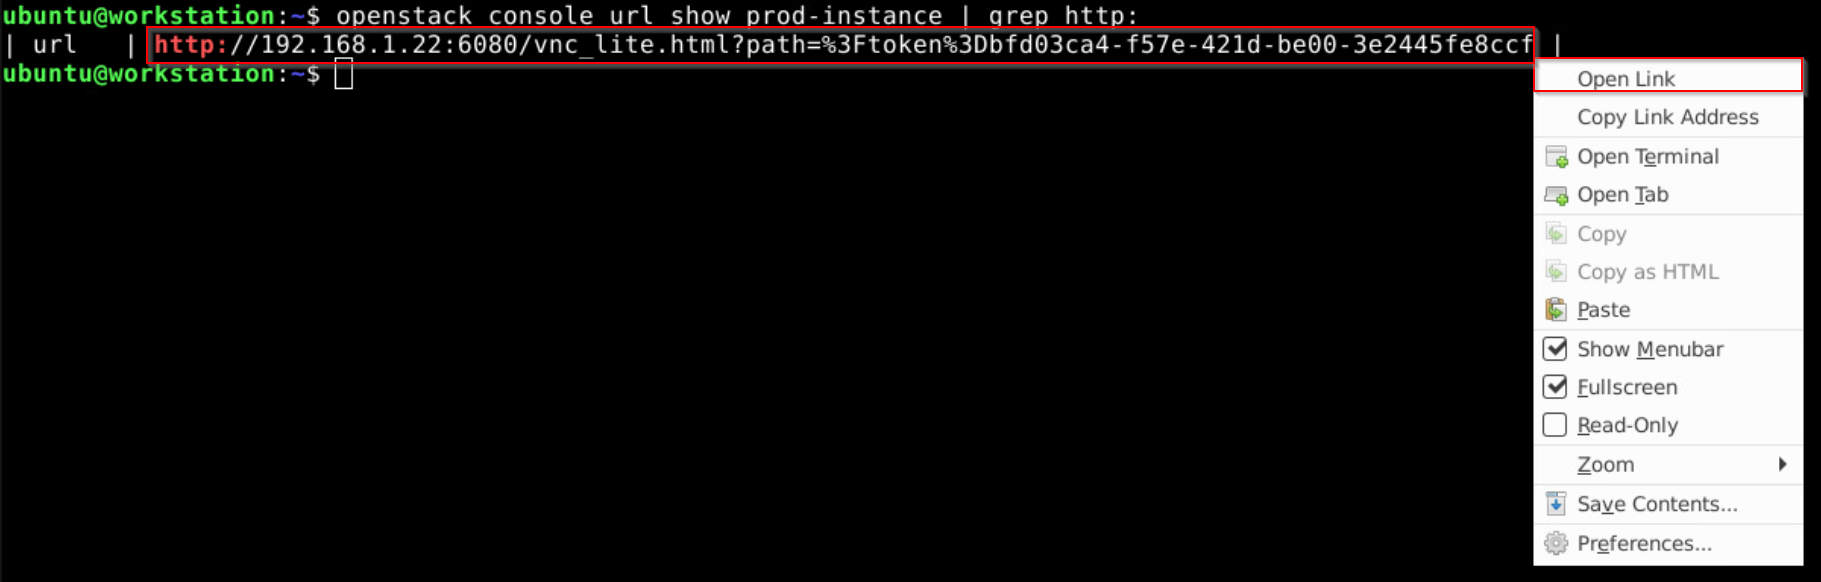
\includegraphics[width=\linewidth]{images/part2/step15.png}
    \end{center}

    \begin{tipbox}
        The UUID for the instance \textbf{prod-instance} can be used in place of \textbf{prod-instance} in the above
        command to identify the instance.
    \end{tipbox}

    \item Enter the command below to display the instance's console URL. Then right click on the URL and select
    \textbf{Open Link}.
    \begin{lstlisting}
        [ubuntu@workstation (keystone-admin)]:~$ openstack console url show prod-instance
    \end{lstlisting}

    \begin{center}
        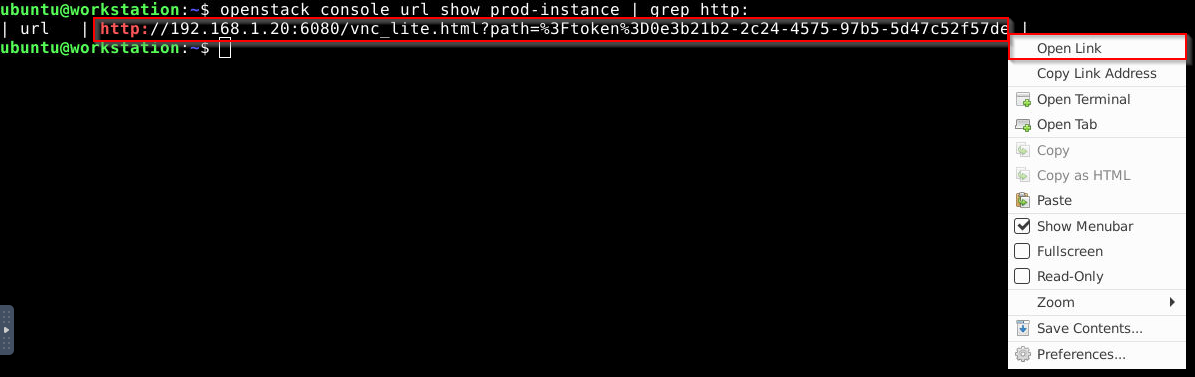
\includegraphics[width=\linewidth]{images/part2/step16.png}
    \end{center}

    \item The web browser will open directly to the instance's console through noVNC. Log into \textbf{prod-instance}
    using \textbf{root} as the username and \textbf{secret} as the password. Then use the \textbf{ping} command to
    verify connectivity with the DHCP server (\textbf{192.168.233.2}).
    \begin{lstlisting}
        $ ping -c3 192.168.233.2
    \end{lstlisting}

    \begin{center}
        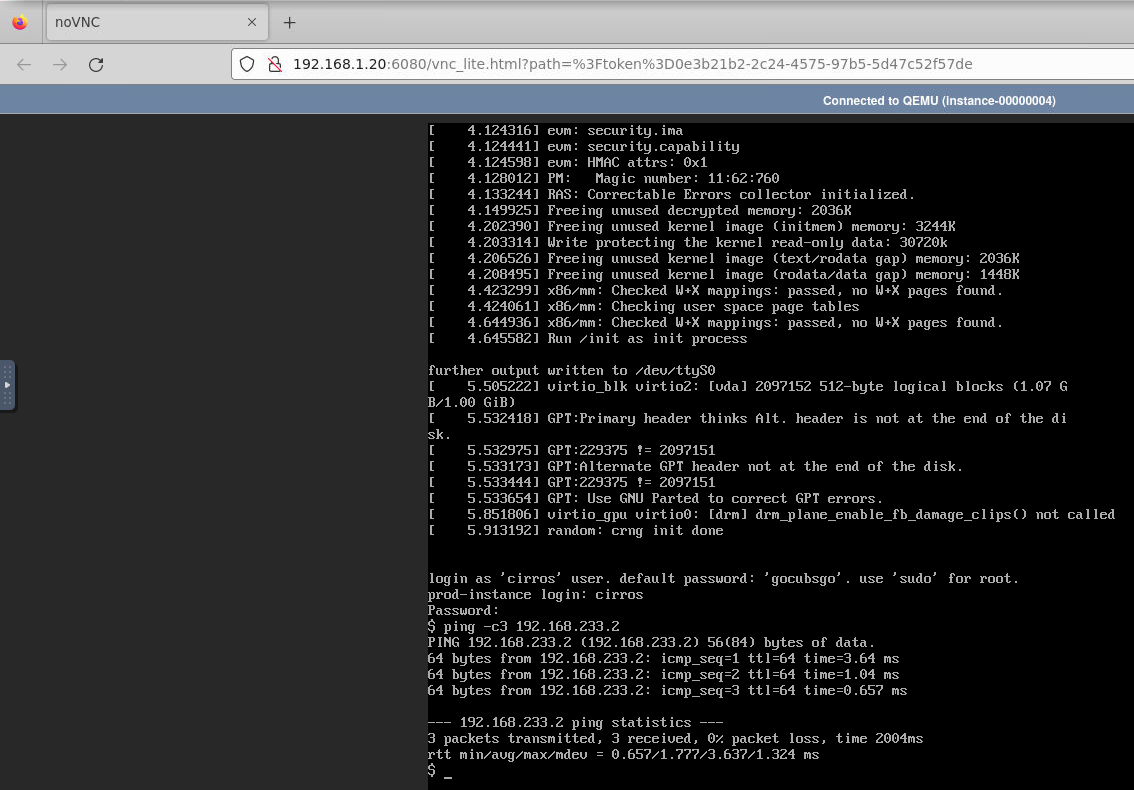
\includegraphics[width=\linewidth]{images/part2/step17.png}
    \end{center}

    \begin{notebox}
        You should receive three successful ping replies.
    \end{notebox}

    \item Close the web browser and change focus back to the previous terminal window.

    \item The instance is now ready to be deleted, but first list the servers so that the effect of the next step can be
    observed.
    \begin{lstlisting}
        [ubuntu@workstation (keystone-admin)]:~$ openstack server list
    \end{lstlisting}

    \begin{center}
        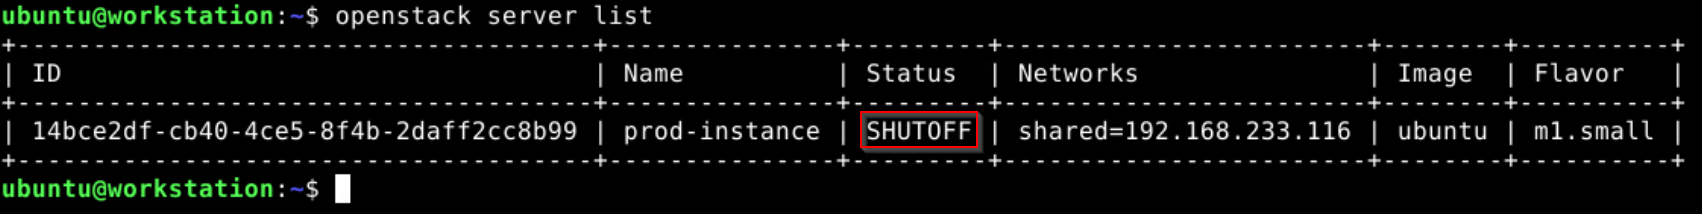
\includegraphics[width=\linewidth]{images/part2/step19.png}
    \end{center}

    \item Enter the command below to delete the instance.
    \begin{lstlisting}
        [ubuntu@workstation (keystone-admin)]:~$ openstack server delete prod-instance
    \end{lstlisting}

    \begin{center}
        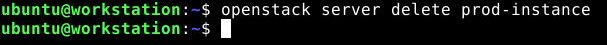
\includegraphics[width=\linewidth]{images/part2/step20.png}
    \end{center}

    \item Ensure that the instance was deleted by seeing that the server list is empty.
    \begin{lstlisting}
        [ubuntu@workstation (keystone-admin)]:~$ openstack server list
    \end{lstlisting}

    \begin{center}
        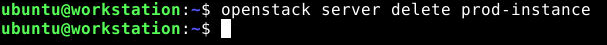
\includegraphics[width=\linewidth]{images/part2/step21.png}
    \end{center}

    \item The lab is now complete.

\end{enumerate}
\end{document}
